\section{Experiments}\label{sec:experiments}
%%%%%%%%%%%%%%%%%%%%%%%%%%%%%%%%%%%%%%%%%%%

The proposed algorithm is part of a python package relying on numpy and numba~\parencite{harris2020,lam2015}.
It will be made open-source upon publication. To compare its efficiency, we used several public datasets described in \cref{table:datasets}.
We performed an extensive benchmark with the following competitors:
\begin{itemize}[noitemsep]
  \item Alternating Direction Method of Multipliers (\texttt{admm})~\parencite{boyd2010}
  \item Anderson acceleration for proximal gradient descent (\texttt{anderson})~\parencite{zhang2020}
  \item Proximal Gradient Descent (\texttt{pgd})~\cite{combettes2005}
  \item Fast Iterative Shrinkage-Thresholding Algorithm (\texttt{fista})~\parencite{beck2009}
  \item Semismooth Newton-Based Augmented Lagrangian (\texttt{newt-alt})~\parencite{Ziyan2019}
  \item The Oracle solver (\texttt{oracle}) uses the clusters obtained via another
        solver to compute coordinate descent updates from the known solver.
  \item The Hybrid (ours) (\texttt{hybrid}) solver (see \cref{alg:hybrid}) combines proximal gradient descent
        and coordinate descent to overcome the non-separability of the SLOPE problem.
\end{itemize}

\begin{table}[]
  \centering
  \label{table:datasets}
  \begin{tabular}{
      l
      S[table-format=6.0,round-mode=off]
      S[table-format=7.0,round-mode=off]
      S[table-format=1.4,round-mode=off]
      c
    }
    \toprule
    Datasets    & \(n\) & \(p\)   & {Density} \\ \midrule
    Simulated 1 & 200   & 20000   & 1         \\
    Simulated 2 & 20000 & 200     & 1         \\
    Simulated 3 & 200   & 2000000 & 0.001     \\
    Rhee2006    & 842   & 361     & ?         \\
    bcTCGA      & 536   & 17322   & 1         \\
    Scheetz2006 & 120   & 18975   & ?         \\ \bottomrule
  \end{tabular}
\end{table}

We used the \texttt{benchopt}~\parencite{moreau2022benchopt} tool to obtain the convergence curves for the different solvers.
\texttt{Benchopt} launches each solver several times increasing the number of iterations and store the objective value, dual gap and time to reach it.
The repository to reproduce the benchmark is available at XXX.

\subsection{Simulated data}

The design matrix $X$ is simulated with correlation between features $j$ and $j'$ equal to $\rho^{|j-j'|}$ where $\rho$ is a parameter that can be chosen in $[0, 1[$.
The true regression vector $\beta^\star$ contains a certain number of non-zero entries that are obtained by simulating a gaussian distribution with zero mean and unit variance.
The observations are equal to $y=X\beta^\star + \varepsilon$ where $\varepsilon$ is a centered gaussian distribution with variance such that $\lVert X\beta^\star\rVert / \lVert \varepsilon \rVert = 3$.

\subsection{Real data}
\klopfe{Do we keep the three different values for $q$ that changes the sequence of lambas?}
\begin{figure*}[htb]
  \centering
  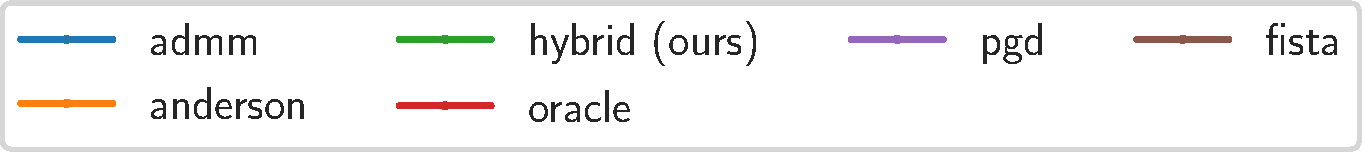
\includegraphics[scale=0.47]{Rhee2006_legend.pdf}
  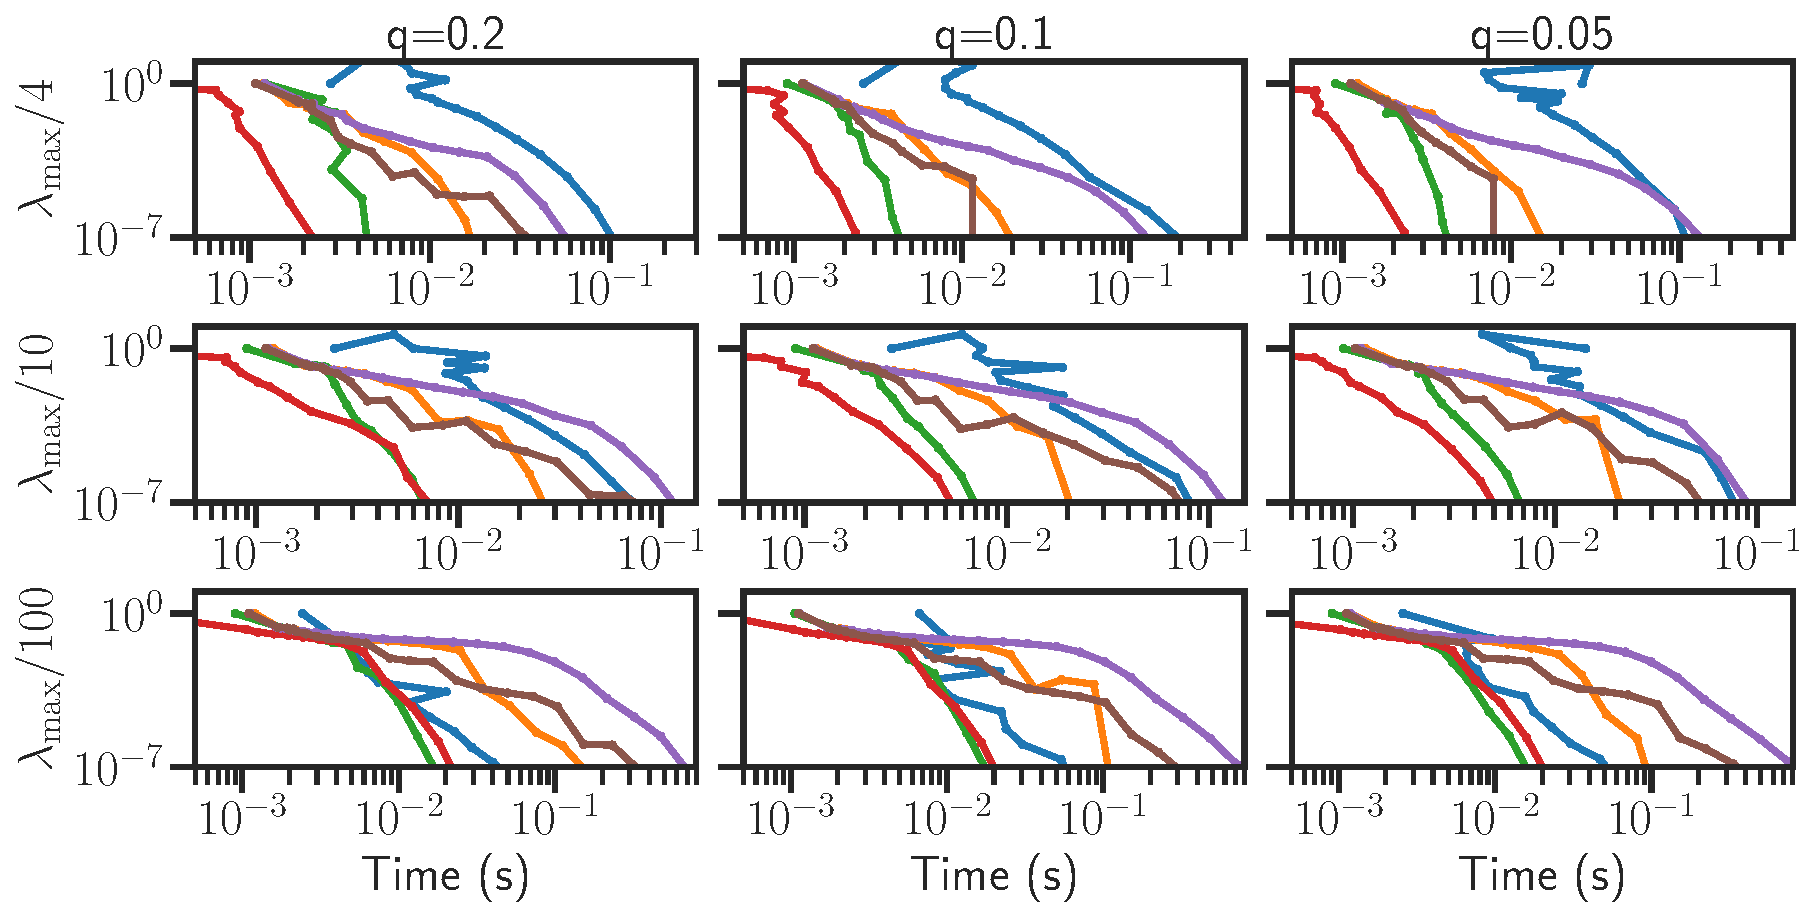
\includegraphics[scale=0.5]{Rhee2006.pdf}
  \caption{Benchmark on the Rhee2006 dataset.}
  \label{fig:Rhee2006}
\end{figure*}
